\subsection{Оценка погрешности}

\subsubsection{Невязка разностной схемы}

\[
  Av = g,\ A - (N + 1) r (N + 1), v, g \in R^{(N + 1)}
\]

Пусть $ v $ - это точное решение разностной схемы, $ u $ -  точное решение дифференциального уравнения, 
$ \tilde{v} $ - полученное решение разностной схемы.

Ищем погрешность решения разностной схемы:
\[
  \varepsilon = \tilde{v} - u
\]

Введем обозначения:
\begin{itemize}
  \item Погрешность решения системы линейных алгебраических уравнений
  \[ z = \tilde{v} - v \]
  \item Погрешность от аппроксимации дифференциального уравнения разностной схемой
  \[ \zeta = v - u \]
  \item Невязка разностной схемы
  \[ \xi = g - Au \]
  \item Невязка алгебраической системы
  \[ r = g - A\tilde{v} \]
\end{itemize}

\subsubsection{Структура погрешности разностной схемы}
\[
  \left\lVert \varepsilon \right\rVert = \left\lVert \tilde{v} - u \right\rVert =
  \left\lVert \tilde{v} - v + v - u \right\rVert = \left\lVert z + \zeta  \right\rVert \leq \left\lVert z \right\rVert
  + \left\lVert \zeta \right\rVert 
\]

Для $\left\lVert \zeta\right\rVert$:
\[
  \xi = g - Au = A(A^{-1}g - u) = A(v - u)
\]
\[
  A\zeta  = \xi
\]

Тем самым погрешность от аппроксимации дифференциального уравнения разностной схемой, связана с невязкой разностной схемы:
\[
  \zeta = A^{-1} \xi 
\]

Для $\left\lVert z \right\rVert$:
\[
  r = g - A\tilde{v} = A(A^{-1}g - \tilde{v}) = A(v - \tilde{v})
\]
\[
  Az = r
\]
Тем самым погрешность решения системы линейных алгебраических уравнений, связана с невязкой алгебраической системы:
\[
  z = A^{-1}r
\]

Подставим в наше неравенство, тем самым получаем:
\[
  \left\lVert \varepsilon \right\rVert \leq \left\lVert A^{-1}r \right\rVert + \left\lVert A^{-1}\xi \right\rVert
  \leq \left\lVert A^{-1} \right\rVert ( \left\lVert r \right\rVert  + \left\lVert \xi \right\rVert)
  \quad \left\lVert A^{-1}\right\rVert  < C
\]

\subsubsection{Вклад от погрешности решения системы алгебраических уравнений}
\[
  \left\lVert z \right\rVert \leq \left\lVert A^{-1} \right\rVert \left\lVert r \right\rVert =
  \left\lVert A \right\rVert \left\lVert A^{-1} \right\rVert \frac{\left\lVert r \right\rVert }{\left\lVert A \right\rVert } 
\]

Знаем что:
\[
  \left\lVert A \right\rVert \geq \frac{\left\lVert g \right\rVert }{\left\lVert v\right\rVert }
\]

Из этого получаем:
\[
  \left\lVert z \right\rVert \leq \left\lVert A \right\rVert \left\lVert A^{-1} \right\rVert
  \frac{\left\lVert r \right\rVert }{\left\lVert A \right\rVert } \left\lVert v \right\rVert 
\]
\[
  cond(A) = \left\lVert A \right\rVert \left\lVert A^{-1} \right\rVert
\]
\[
  \frac{\left\lVert r \right\rVert }{\left\lVert A \right\rVert } \sim \varepsilon_{M}
\]


\[
  \left\lVert z \right\rVert \leq cond(A) \varepsilon_{M} \left\lVert v \right\rVert 
\]

\subsubsection{Разложение невязки}

Разностная схема

\[
  -\left[ \frac{1}{r} \frac{d}{dr} \left(rk\frac{du}{dr} \right)\ -\ qu(r) \right] = f_i
\]
\[
  -\left[ \frac{d}{dr} \left(rk\frac{du}{dr} \right)\ -\ rqu(r) \right] = rf_i
\]

Введем новые обозначения:
\begin{center}
  $ \tilde{k} = rk \qquad \tilde{q} = rq \qquad \tilde{f} = rf $
\end{center}

Получим:
\[
  -\left[ \frac{d}{dr} \left(\tilde{k}\frac{du}{dr} \right)\ -\ \tilde{q}u(r) \right] = \tilde{f}_i
\]

Еще раз напишем разностную схему:
\[
  -\left[ \tilde{k}_{i+0.5}\frac{u_{i+1}-u_i}{h} + \nu_1 - \frac{h}{2} \tilde{q}_i v_i \right]\ =\ \frac{h}{2} \tilde{f}_i \quad i = 0
\]
\[
-\left[ \tilde{k}_{i+0.5}\frac{u_{i+1}-u_i}{h} - \tilde{k}_{i-0.5}\frac{u_{i} - u_{i-1}}{h} - h \tilde{q}_i v_i\right]\ =\ h \tilde{f}_i \quad i = 1, 2, ..., N -1
\]
\[
-\left[ \nu_2 - \tilde{k}_{i-0.5} \cdot \frac{u_i-u_{i-1}}{h}- \frac{h}{2} \tilde{q}_i v_i \right]\ =\ \frac{h}{2} \tilde{f}_i \quad i = N
\]

На левой границе интервала уравнение для невзяки выглядит следующим образом:
\[
  \xi_i = \frac{h}{2} \tilde{f}_i + \left [ \tilde{k}_{i+0.5}\frac{u_{i+1}-u_i}{h} + \nu_1 - \frac{h}{2} \tilde{q}_i u_i \right ]
\]

Внутри интервала:
\[
  \xi_i = h \tilde{f}_i + \left [ \tilde{k}_{i+0.5}\frac{u_{i+1}-u_i}{h} - \tilde{k}_{i-0.5}\frac{u_{i} - u_{i-1}}{h} - h \tilde{q}_i u_i \right ]
\]

На правой границе:
\[
  \xi_i = \frac{h}{2} \tilde{f}_i + \left [ \nu_2 - \tilde{k}_{i-0.5}\frac{u_{i} - u_{i-1}}{h} -  \frac{h}{2} \tilde{q}_i u_i \right ]
\]

Найдем разложение разностной схемы

\[
  u_i = u(x_i + h) = u_i + h \frac{d u_i}{d r} + \frac{h^2 }{2} \frac{d^2 u_i}{d r^2}
  + \frac{h^3 }{6} \frac{d^4 u_i}{d r^3} + \frac{h^4 }{24} \frac{d^4 u_i}{d r^4} + \mathcal{O}(h^5)
\]
\[
  \frac{u_{i + 1} - u_{i}}{h} = \frac{d u_i}{dr} + \frac{h}{2} \frac{d^2 u_i}{dr^2} 
  + \frac{h^2}{6}\frac{d^3 u_i}{dr^3} + \frac{h^3}{24}\frac{d^4 u_i}{dr^4} + \mathcal{O}(h^4)
\]
\[
  \tilde{k}_{i+\frac{1}{2}} = \tilde{k}(x_i + \frac{h}{2}) = \tilde{k_i} + \frac{h^2 }{2}\frac{d \tilde{k_i}}{d r} + \frac{h^2 }{8}\frac{d^2 \tilde{k_i}}{d r^2}
  + \frac{h^3 }{48}\frac{d^3 \tilde{k_i}}{d r^3} + \mathcal{O}(h^3)
\]
Получаем:
\begin{align*}
  \tilde{k}_{i+\frac{1}{2}} \frac{u_{i + 1} - u_{i}}{h} = &\tilde{k_i} \frac{du_i}{dr} \\
  &+ h \left [ \frac{1}{2}\tilde{k_i} \frac{d^2 u_i}{d r^2} + \frac{1}{2}\frac{d \tilde{k}_i}{dr} \frac{d u_i}{d r} \right ] \\
  &+ h^2 \left [ \frac{1}{6}\tilde{k_i} \frac{d^3 u_i}{d r^3} + \frac{1}{4}\frac{d \tilde{k}_i}{dr} \frac{d^2 u_i}{d r^2} + \frac{1}{8}\frac{d^2 \tilde{k_i}}{dr^2} \frac{d u_i}{d r} \right ] \\
  &+ h^3 \left [ \frac{1}{24}\tilde{k_i} \frac{d^4 u_i}{d r^4} + \frac{1}{12}\frac{d \tilde{k_i}}{dr} \frac{d^3 u_i}{d r^3} + \frac{1}{16}\frac{d^2 \tilde{k_i}}{dr^2} \frac{d^2 u_i}{d r^2} + \frac{1}{48}\frac{d^3 \tilde{k_i}}{dr^3} \frac{d u_i}{d r}\right ] \\
  &+ \mathcal{O}(h^4)
\end{align*}

\[
  u_{i-1} = u(x_i - h) = u_i - h \frac{d u_i}{d r} + \frac{h^2 }{2} \frac{d^2 u_i}{d r^2}
  - \frac{h^3 }{6} \frac{d^4 u_i}{d r^3} + \frac{h^4 }{24} \frac{d^4 u_i}{d r^4} + \mathcal{O}(h^5)
\]
\[
  \frac{u_{i} - u_{i-1}}{h} = \frac{d u_i}{dr} - \frac{h}{2} \frac{d^2 u_i}{dr^2} 
  + \frac{h^2}{6}\frac{d^3 u_i}{dr^3} - \frac{h^3}{24}\frac{d^4 u_i}{dr^4} + \mathcal{O}(h^4)
\]
\[
  \tilde{k}_{i-\frac{1}{2}} = \tilde{k}(x_i - \frac{h}{2}) = \tilde{k_i} - \frac{h^2 }{2}\frac{d \tilde{k_i}}{d r} + \frac{h^2 }{8}\frac{d^2 \tilde{k_i}}{d r^2}
  - \frac{h^3 }{48}\frac{d^3 \tilde{k_i}}{d r^3} + \mathcal{O}(h^3)
\]
Получаем:
\begin{align*}
  \tilde{k}_{i-\frac{1}{2}} \frac{u_{i} - u_{i-1}}{h} = &\tilde{k_i} \frac{du_i}{dr} \\
  &- h \left [ \frac{1}{2}\tilde{k_i} \frac{d^2 u_i}{d r^2} + \frac{1}{2}\frac{d \tilde{k}_i}{dr} \frac{d u_i}{d r} \right ] \\
  &+ h^2 \left [ \frac{1}{6}\tilde{k_i} \frac{d^3 u_i}{d r^3} + \frac{1}{4}\frac{d \tilde{k}_i}{dr} \frac{d^2 u_i}{d r^2} + \frac{1}{8}\frac{d^2 \tilde{k_i}}{dr^2} \frac{d u_i}{d r} \right ] \\
  &- h^3 \left [ \frac{1}{24}\tilde{k_i} \frac{d^4 u_i}{d r^4} + \frac{1}{12}\frac{d \tilde{k_i}}{dr} \frac{d^3 u_i}{d r^3} + \frac{1}{16}\frac{d^2 \tilde{k_i}}{dr^2} \frac{d^2 u_i}{d r^2} + \frac{1}{48}\frac{d^3 \tilde{k_i}}{dr^3} \frac{d u_i}{d r}\right ] \\
  &+ \mathcal{O}(h^4)
\end{align*}

Подставим это в уравнение невязки внутри интервала:
\begin{align*}
  \xi_i = h \tilde{f}_i +
  &\left [ \tilde{k_i} \frac{du_i}{dr} \right . + h \left [ \frac{1}{2}\tilde{k_i} \frac{d^2 u_i}{d r^2} + \frac{1}{2}\frac{dk_i}{dr} \frac{d u_i}{d r} \right ] 
    + h^2 \left [ \frac{1}{6}\tilde{k_i} \frac{d^3 u_i}{d r^3} + \frac{1}{4}\frac{dk_i}{dr} \frac{d^2 u_i}{d r^2} + \frac{1}{8}\frac{d^2 \tilde{k_i}}{dr^2} \frac{d u_i}{d r} \right ] \\
    &+ h^3 \left [ \frac{1}{24}\tilde{k_i} \frac{d^4 u_i}{d r^4} + \frac{1}{12}\frac{d \tilde{k_i}}{dr} \frac{d^3 u_i}{d r^3} + \frac{1}{16}\frac{d^2 \tilde{k_i}}{dr^2} \frac{d^2 u_i}{d r^2} + \frac{1}{48}\frac{d^3 \tilde{k_i}}{dr^3} \frac{d u_i}{d r} \right ] \\
    &- \tilde{k_i} \frac{du_i}{dr} + h \left [ \frac{1}{2}\tilde{k_i} \frac{d^2 u_i}{d r^2} + \frac{1}{2}\frac{dk_i}{dr} \frac{d u_i}{d r} \right ] \\
    &- h^2 \left [ \frac{1}{6}\tilde{k_i} \frac{d^3 u_i}{d r^3} + \frac{1}{4}\frac{dk_i}{dr} \frac{d^2 u_i}{d r^2} + \frac{1}{8}\frac{d^2 \tilde{k_i}}{dr^2} \frac{d u_i}{d r} \right ] \\
    &- h^3 \left [ \frac{1}{24}\tilde{k_i} \frac{d^4 u_i}{d r^4} + \frac{1}{12}\frac{d \tilde{k_i}}{dr} \frac{d^3 u_i}{d r^3} + \frac{1}{16}\frac{d^2 \tilde{k_i}}{dr^2} \frac{d^2 u_i}{d r^2} + \frac{1}{48}\frac{d^3 \tilde{k_i}}{dr^3} \left . \frac{d u_i}{d r}\right ] \right ]
\end{align*}

Приводим подобные слагаемые:
\begin{align*}
  \xi_i = &h \left [ \tilde{f} + \tilde{k} \frac{d^2u}{dr^2} \frac{d\tilde{k}}{dr}\frac{du}{dr} - \tilde{q}u \right ] \\
  &+ h^3 \left[ \frac{1}{12}\tilde{k} \frac{d^4 u_i}{d r^4}  + \frac{1}{6} \frac{d \tilde{k}}{dr} \frac{d^3 u_i}{d r^3} 
  + \frac{1}{8} \frac{d^2 \tilde{k}}{dr^2} \frac{d^3 u_i}{d r^3} + \frac{1}{24} \frac{d^3 \tilde{k}}{dr^3} \frac{d u_i}{d r} 
  \right] + \mathcal{O}(h^4)
\end{align*}

Можно заметить что:
\[
  \left [ \tilde{k} \frac{d^2u}{dr^2} + \frac{d\tilde{k}}{dr}\frac{du}{dr} \right ] =
  \frac{d}{dr}\left ( \tilde{k} \frac{du}{dr} \right )
\]

При этом:
\[
  \tilde{f} + \frac{d}{dr}\left ( \tilde{k} \frac{du}{dr} \right ) - \tilde{q}u = 0
\]

Тем самым получаем:
\begin{align*}
  \xi_i = h^3 \left[ \frac{1}{12}\tilde{k} \frac{d^4 u_i}{d r^4}  + \frac{1}{6} \frac{d \tilde{k}}{dr} \frac{d^3 u_i}{d r^3} 
  + \frac{1}{8} \frac{d^2 \tilde{k}}{dr^2} \frac{d^3 u_i}{d r^3} + \frac{1}{24} \frac{d^3 \tilde{k}}{dr^3} \frac{d u_i}{d r} 
  \right] + \mathcal{O}(h^4)
\end{align*}

Найдем разложение невязки для граничного условия слева:
\[
  \xi_i = \frac{h}{2} \tilde{f}_i + \left [ \tilde{k}_{i+0.5}\frac{u_{i+1}-u_i}{h} + \nu_1 - \frac{h}{2} \tilde{q}_i u_i \right ] \quad i = 0
\]

Получаем:
\begin{align*}
  \xi_i = &\frac{h}{2} \tilde{f}_i + \tilde{k_i} \frac{du_i}{dr} + h \left [ \frac{1}{2}\tilde{k_i} \frac{d^2 u_i}{d r^2} + \frac{1}{2}\frac{d \tilde{k}_i}{dr} \frac{d u_i}{d r} \right ] \\
  &+ h^2 \left [ \frac{1}{6}\tilde{k_i} \frac{d^3 u_i}{d r^3} + \frac{1}{4}\frac{d \tilde{k}_i}{dr} \frac{d^2 u_i}{d r^2} + \frac{1}{8}\frac{d^2 \tilde{k_i}}{dr^2} \frac{d u_i}{d r} \right ]
  + \mathcal{O}(h^3) + \nu_1 - \frac{h}{2} \tilde{q}_i u_i
\end{align*}

Сгруппируем слагаемые при одинаковых степенях h:
\begin{align*}
  \xi_i = & h^0 \left[ \nu_1 + \tilde{k_i} \frac{du_i}{dr}\right]
  + \frac{h}{2} \left[ \tilde{f}_i + \tilde{k_i} \frac{d^2 u_i}{d r^2} + \frac{d \tilde{k}_i}{dr} \frac{d u_i}{d r} - \tilde{q}_i u_i \right] \\
  &+ h^2 \left [ \frac{1}{6}\tilde{k_i} \frac{d^3 u_i}{d r^3} + \frac{1}{4}\frac{d \tilde{k}_i}{dr} \frac{d^2 u_i}{d r^2} + \frac{1}{8}\frac{d^2 \tilde{k_i}}{dr^2} \frac{d u_i}{d r} \right ] + \mathcal{O}(h^3)
\end{align*}

Из условия:
\[
  k \left. \frac{du}{dr}\right\vert_{r = R_L} = -\nu _1
\]

Также:
\[
  \left [ \tilde{k} \frac{d^2u}{dr^2} + \frac{d\tilde{k}}{dr}\frac{du}{dr} \right ] =
  \frac{d}{dr}\left ( \tilde{k} \frac{du}{dr} \right )
\]
\[
  \tilde{f} + \frac{d}{dr}\left ( \tilde{k} \frac{du}{dr} \right ) - \tilde{q}u = 0
\]

Тем самым получаем:
\begin{align*}
  \xi_i = h^2 \left [ \frac{1}{6}\tilde{k_i} \frac{d^3 u_i}{d r^3} + \frac{1}{4}\frac{d \tilde{k}_i}{dr} \frac{d^2 u_i}{d r^2} + \frac{1}{8}\frac{d^2 \tilde{k_i}}{dr^2} \frac{d u_i}{d r} \right ] + \mathcal{O}(h^3)
\end{align*}

Теперь найдем разложение невязки для правой границы
\[
  \xi_i = \frac{h}{2} \tilde{f}_i + \left [ \nu_2 - \tilde{k}_{i-0.5}\frac{u_{i} - u_{i-1}}{h} - \frac{h}{2} \tilde{q}_i u_i \right ], \quad i = N
\]

Получаем:
\begin{align*}
  \xi_i = &\frac{h}{2} \tilde{f}_i - \tilde{k_i} \frac{du_i}{dr} + h \left [ \frac{1}{2}\tilde{k_i} \frac{d^2 u_i}{d r^2} + \frac{1}{2}\frac{d \tilde{k}_i}{dr} \frac{d u_i}{d r} \right ] \\
  &- h^2 \left [ \frac{1}{6}\tilde{k_i} \frac{d^3 u_i}{d r^3} + \frac{1}{4}\frac{d \tilde{k}_i}{dr} \frac{d^2 u_i}{d r^2} + \frac{1}{8}\frac{d^2 \tilde{k_i}}{dr^2} \frac{d u_i}{d r} \right ]
  + \mathcal{O}(h^3) + \nu_2 - \frac{h}{2} \tilde{q}_i u_i
\end{align*}

Сгруппируем слагаемые при одинаковых степенях h:
\begin{align*}
  \xi_i = &h^0 \left[ \nu_2 - \tilde{k_i} \frac{du_i}{dr} \right] + \frac{h}{2} \left[ \tilde{f}_i + \tilde{k_i} \frac{d^2 u_i}{d r^2} + \frac{d \tilde{k}_i}{dr} \frac{d u_i}{d r} - \tilde{q}_i u_i\right] \\
  &- h^2 \left [ \frac{1}{6}\tilde{k_i} \frac{d^3 u_i}{d r^3} + \frac{1}{4}\frac{d \tilde{k}_i}{dr} \frac{d^2 u_i}{d r^2} + \frac{1}{8}\frac{d^2 \tilde{k_i}}{dr^2} \frac{d u_i}{d r} \right ] + \mathcal{O}(h^3)
\end{align*}

Из условия:
\[
  -k \left. \frac{du}{dr}\right\vert_{r = R_R}\ =\ -\nu_2
\]

Также:
\[
  \left [ \tilde{k} \frac{d^2u}{dr^2} + \frac{d\tilde{k}}{dr}\frac{du}{dr} \right ] =
  \frac{d}{dr}\left ( \tilde{k} \frac{du}{dr} \right )
\]
\[
  \tilde{f} + \frac{d}{dr}\left ( \tilde{k} \frac{du}{dr} \right ) - \tilde{q}u = 0
\]

Тем самым получаем:
\begin{align*}
  \xi_i = - h^2 \left [ \frac{1}{6}\tilde{k_i} \frac{d^3 u_i}{d r^3} + \frac{1}{4}\frac{d \tilde{k}_i}{dr} \frac{d^2 u_i}{d r^2} + \frac{1}{8}\frac{d^2 \tilde{k_i}}{dr^2} \frac{d u_i}{d r} \right ] + \mathcal{O}(h^3)
\end{align*}

\subsubsection{Зависимость погрешности от числа разбиений}

Как было показано выше, невязка $\left\lVert \xi \right\rVert \sim h^2$, 
когда погрешность решения системы алгебраических уравнений $ \left\lVert z \right\rVert \sim \frac{1}{h^2} $.
\begin{center}
  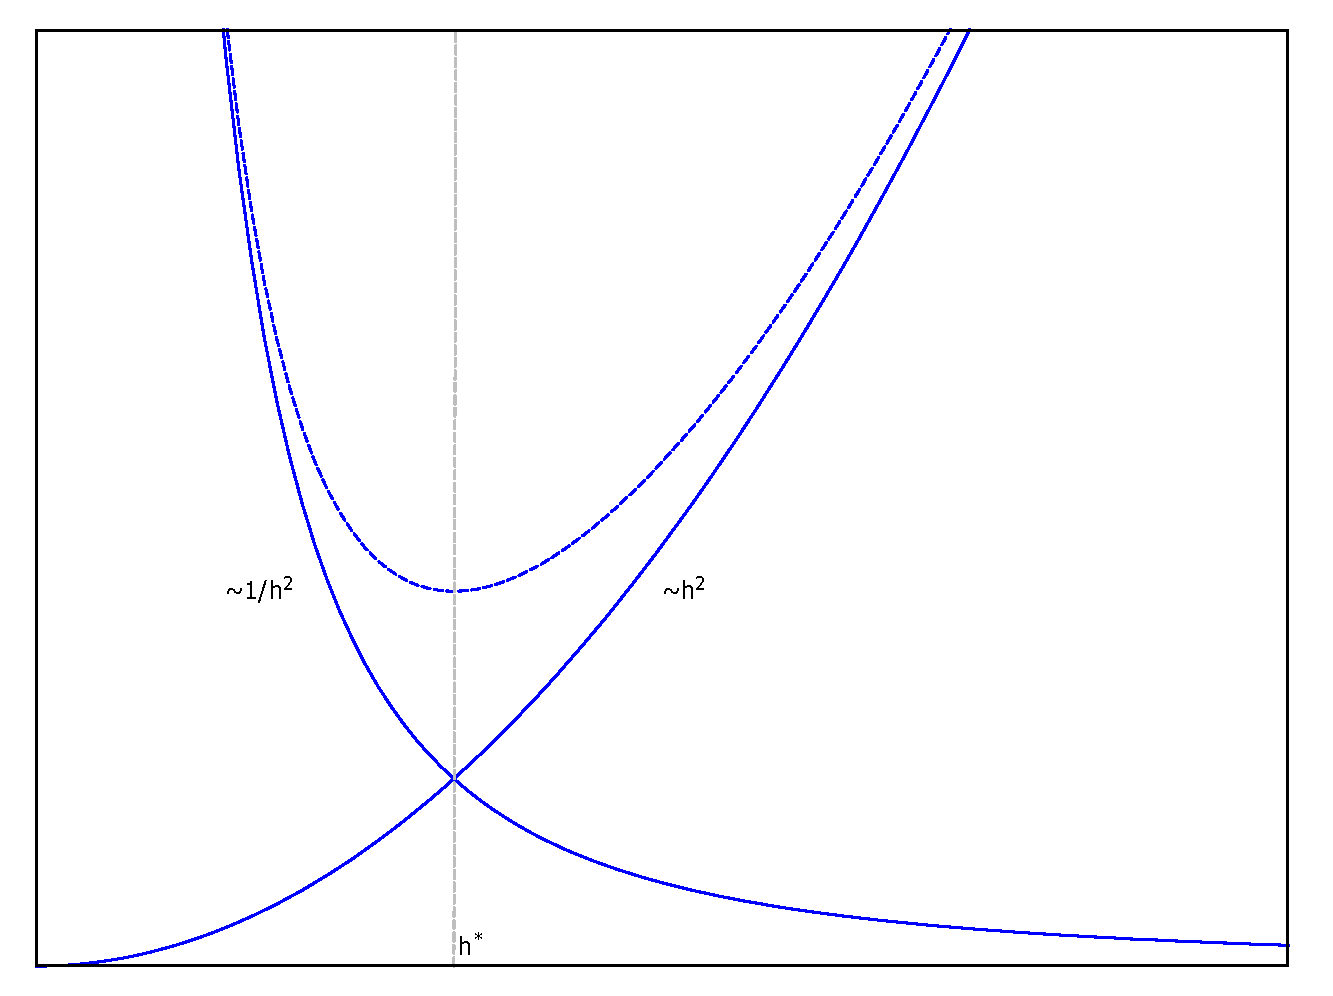
\includegraphics[width=0.7\textwidth]{img/err.pdf}
\end{center}

Значит существует такое число разбиений где погрешность минимальная.